\documentclass[main.tex]{subfiles}

\begin{document}

\section{Landmarks}

Before implementing a system that uses landmarks, the options for potential landmarks first have to be analysed as to whether they can provide the benefits in our specific environment. The main options that were explored are:

\begin{itemize}
	\item Stairs
	\item Elevators
	\item Areas of unique magnetic readings
	\item Wi-fi Routers
\end{itemize}

The first 2 options are present in the department building, however they are limited in how they can help with resetting the error in the system. This is because stairs and elevators are naturally only used when moving from one floor to another. Meaning navigation on a single floor will not be helped with resetting error but for navigation over multiple floors they can be utilised. 

Both have unique patterns that can be seen from the accelerometer readings, in conjunction with the potential for the barometer to verify the movement between floors, they can be used as landmarks. However a detection algorithm did not get implemented for either of the patterns, to still allow for the removal of error build up the user is requested to alert the application when they have moved from one floor to another.

Magnetic readings are likely to be prevelant throughout our environment as the entire building has lots of electronic equipment, such as computers, servers, etc.... These readings manifest themselves more in general magnetic inteference as appose to small pockets of unique signals, this makes areas of magnetic readings unfeasible as a landmark in our scenario.

This leaves Wi-fi as the only method of removing error when navigating within a floor, to do this all the routers on a floor need to be identified.

\begin{center}
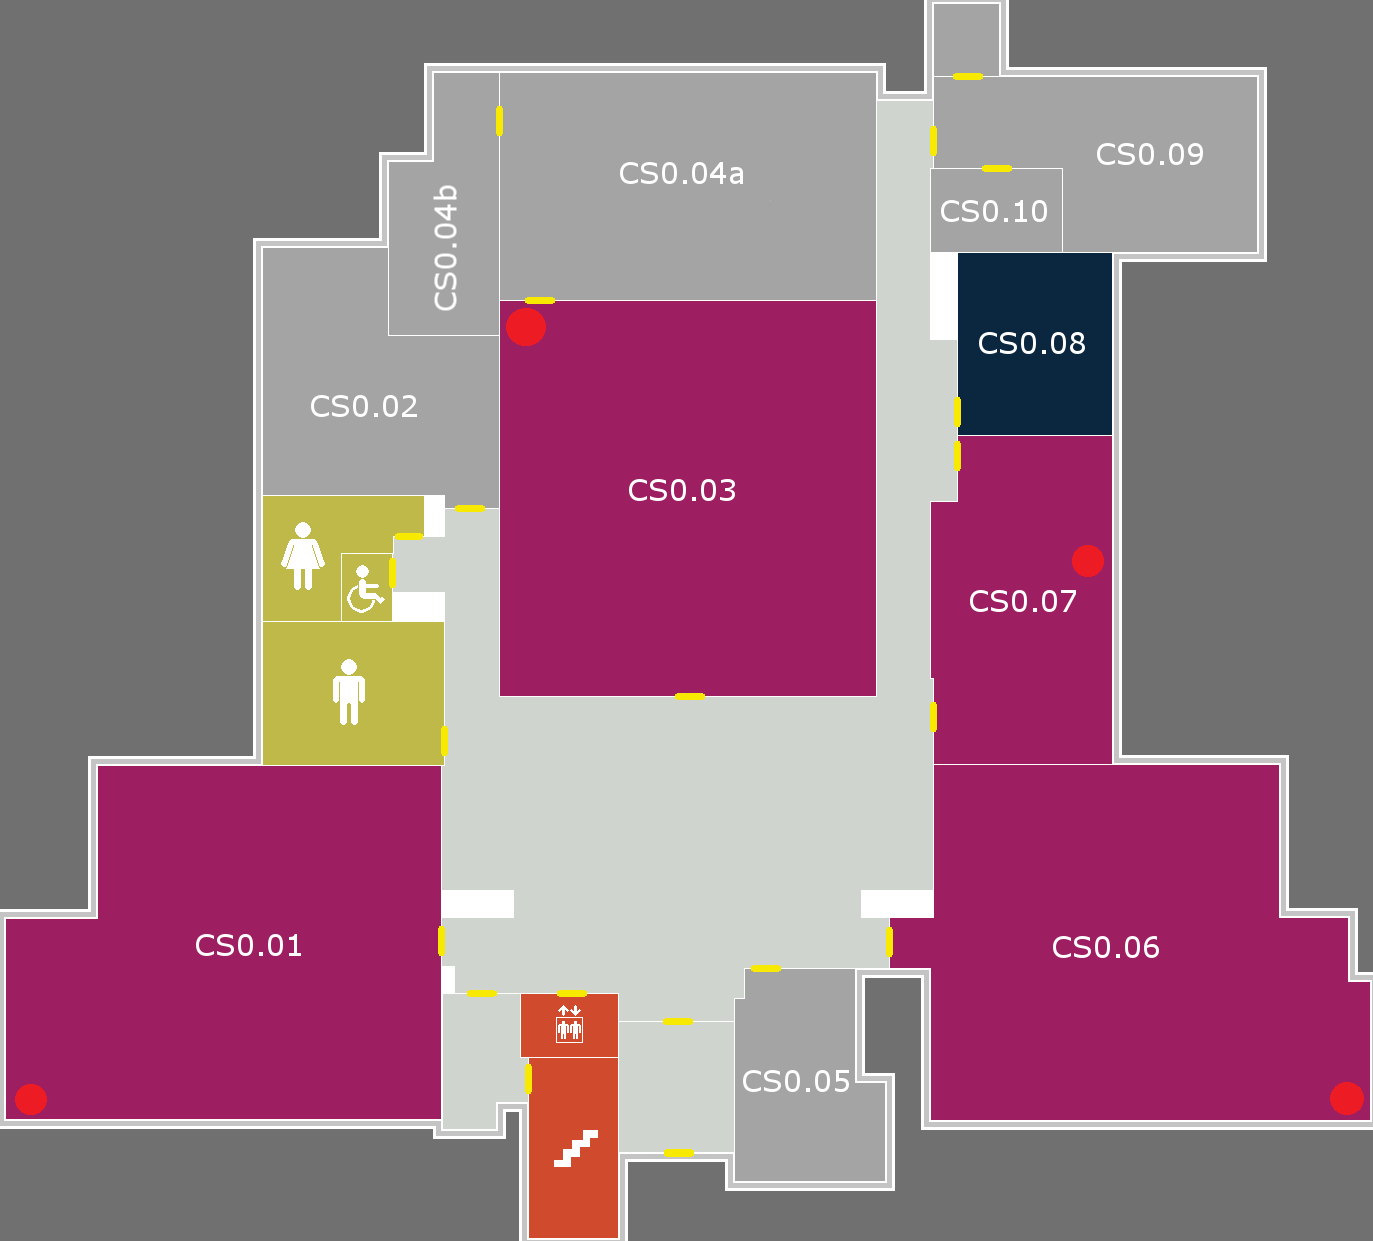
\includegraphics[scale=0.3]{images-implementation/wifiLocation.png}
\captionof{figure}{The location of Wifi routers on the ground floor of DCS, marked as red dots}
\label{fig:wifiLoc}
\end{center}

After identifying the locations of the routers on the ground floor, as shown in Figure~\ref{fig:wifiLoc}, it becomes apparent that bar one they will not be able to serve as landmarks. They reside with in the corners/sides of the rooms, and for a landmark to be useful the user must path close enough to it for it to be a viable choice for resetting error. With most of their locations it is impossible for an effecient routing algorithm to return a path in which the routers are not either at the start or the end of the route. Hence making them effectively useless for this purpose. The singular router that could be used is the one residing within CS0.03, as it sits before a door that leads to two other rooms. Despite this ideal placement it still isn't suited for use as a Landmark, as the two rooms for which the pathing would make the user pass by the router have restricted access due to containing servers/equipment.

We also found that we often picked up routers from different floors in certian areas, whilst this could be a landmark in a similar way to pockets of magnetic readings. It was not consistent across different devices used for testing, hence not viable for a landmark since it isn't available to all. As well as this devices would connect to a room's router outside of them, meaning that connecting to a router that is specific to a large room it is an unreliable to assume the user is within it.

Whilst routers are not viable for landmarks on the ground floor for the reasons stated above, it doesn't mean they will not be viable for the upper floors. This was tested the same as before by identifying router locations, but it became quickly evident that from placement again they would not be of use. In conjunction with the large number of small rooms/offices on the upper floors it becomes hard to snap a user to these routers.

Another thing to note about using routers is that there are two main bands that are used for communication, 2Ghz and 5Ghz, so dependent on the routers and smartphones they may not be usable. In this case the router's in the department are dualband meaning both are available, it does however mean that 2 MAC addresses are needed to be stored per router for unique identification.

Overall having looked at these landmarks it is clear that all of these options could be useful in the right environment, unfortunately in our case a variety of factors play a role in making them infeasible.

\section{Barometer}

For the barometer, both Andriod and iOS have native ways to get both the current air pressure and the height above sea level the device. From research and small amounts of testing it was evident that using the absolute height would not provide any useful way of detecting floor change with the fluctuations that occur with time, weather and location. To avoid this the difference between heights can be used to detect if a user has gone up or down a floor. 

However despite there being a clear correlation between moving between floors and the change in height, the height recieved from these native functions would range between 3-5m over a small period of time. This means that it is very difficult to be certain if the user has changed floors, the difference in floor height with in the department is 4m, or it is simply an outlier from the functions. 

To help combat this the average was taken over a large number of reading across a period of time, however whilst this solved the rapidly changing value, it meant that if a user took too long transistioning between floors the average would slowly slide in their direction of movement. When this occurs nothing will be flagged as a large enough distance to be moving from floor A to B and the system will not recognise the movement. 

Given more time this issues could be solved, and from research and the testing done it can be seen that the barometer will be a useful sensor for indoor localisation.

\end{document}